\section{Diagrammes incontournables}
\subsection{Diagramme d’activité du processus de Gestion des prêts dans la bibliothèque}
\paragraph{}
\begin{figure}[h]
        \centering
        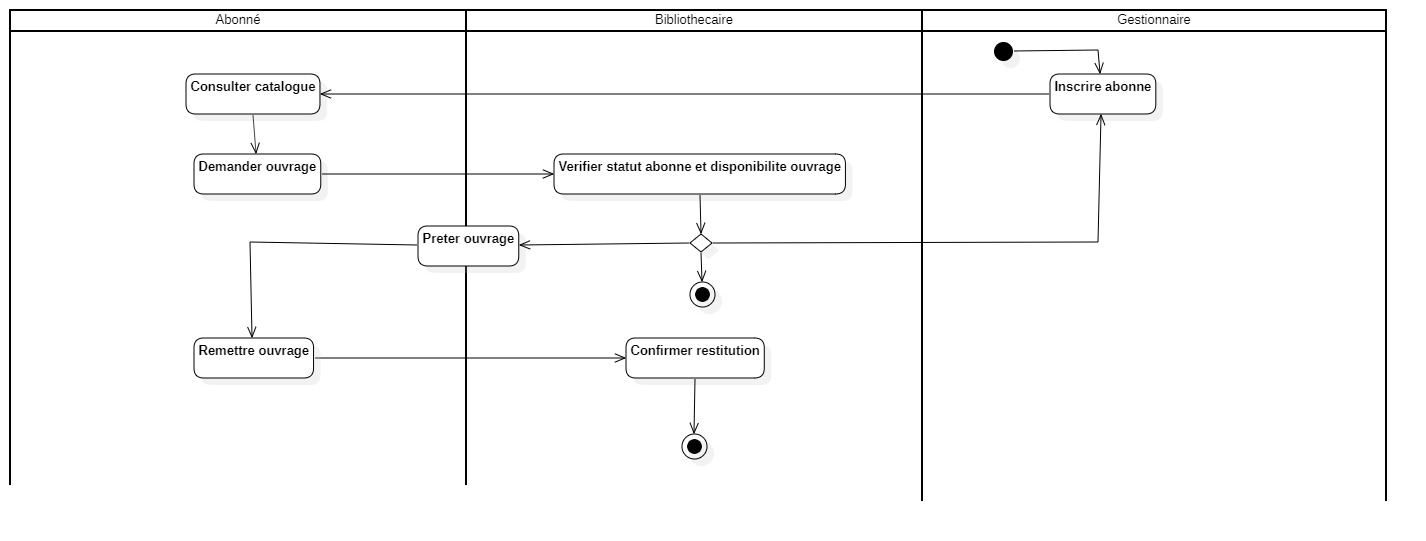
\includegraphics[width=1\textwidth]{ActivityDiagram1}
        \caption{Diagramme d’activité du processus de Gestion des prêts dans la bibliothèque}
        \label{image-ActivityDiagram1}
        \end{figure}
\par
Les prêts au sein de la bibliothèque universitaire suivent un ensemble d'étapes précis.
Certaines contraintes sont donc à respecter continuellement. Pour commencer, n'importe qui 
peut consulter la liste des ouvrages accessibles dans la biblio. Mais pour savoir quel 
ouvrage est disponible au moment de la recherche, il faut que le gestionnaire enregistre 
l'abonné. De son côté, il faut que le bibliothécaire enregistre les ouvrages acquis 
dans la base de données du système. \par 
Après s'être assuré de la disponibilité d'un livre, l'abonné peut alors se rendre sur 
place pour effectuer l'emprunt. Du coup, le bibliothèque a pour responsabilité de relever
toutes les informations relatives à l'emprunt en question. Certains champs sont obligatoires
et le système renverra un message d'erreur s'ils ne sont pas remplis. Si l'abonné a déjà 
trois livres en sa possession, le système n'autorise pas la validation de l'emprunt.
Une fois l'emprunt validé, l'abonné peut vaquer à ses occupations sans problème. Il lui 
est donné trois semaines pour rester en possession du livre. De façon exceptionnelle, il 
peut pourtant le garder durant cinq semaines. Pourtant, une fois ce délai atteint, le 
système envoie une relance automatique sur le mail du concerné pour le rappeler qu'il doit 
rapporter ce livre en question.
Lorsque l'abonné rend le livre, il se présente encore une fois à la bibliothèque et le 
responsable se charge de modifier l'emprunt en y ajoutant une date de restitution. \par 
Ainsi se déroule le cycle de la gestion des emprunts au sein de la bibliothèque.
\subsection{Diagramme de classe de gestion des prêts}
\paragraph{}

Ce diagramme est utile pour présenter les différentes classes ainsi que les relations 
entre elles. Il est obligatoire lors d'une modélisation. Selon certaines sources, il 
s'agit d'un document indispensable sui représente la vue de conception statique 
d'un système. Il serait donc impensable de concevoir l'application sans prendre le temps 
d'implémenter cet outil.
\par 
Il se présente de la sorte: \par 
\begin{figure}[h]
        \centering
        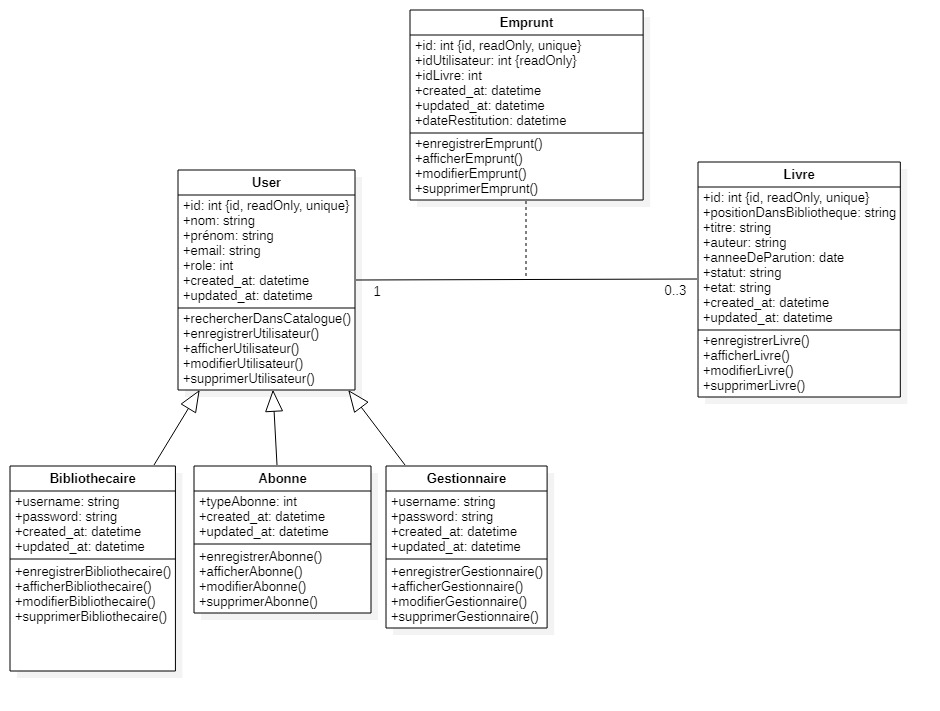
\includegraphics[width=1\textwidth]{ClassDiagram1}
        \caption{Diagramme de classe de gestion des prêts}
        \label{image-ClassDiagram1}
        \end{figure}
\par